
\subsection{Verification}
\label{subsec:verification}


In this subsection, we will show the validity of our method by testing on various 3D models.


\paragraph{Object as a unit elastic body}
In seeking the optimal architecture for 3D objects, the frame structure with assumptions from Section~\ref{subsec:frame} is adopted.
However, in practical 3D printing, the struts inside the object are not linked together by joints;
they are shaped by dissolving the printing material into a unit body.
Thus, we need to confirm the strain and stress distribution of the object by taking the object as an elastic body, for which the deformations from tensile force, sheer force, and even torsion force, are all considered.



For an elastic body $\Omega$, the stionary state of objects under forces can be described by the linear elasticity problem,
\begin{align}\label{eq:linear-elasticity}
     -\mbox{div}(\sigma(\epsilon(u))) & = f, \quad in\ \Omega \notag \\
                             u & = 0, \quad on\ \Gamma_D \\
          \sigma(\epsilon(u))\cdot n & = g, \quad on\ \Gamma_N. \notag
\end{align}
In this problem, $u$ is displacement, $\epsilon(u)=1/2(\nabla u+\nabla u^T)$ is the strain,
and $\sigma(\epsilon)=2\mu\epsilon+\gamma(\mathrm{tr}(\epsilon))I$ is the stress.
The quantities $\gamma$ and $\mu$ are the Lame moduli of the material. Such a problem can be solved by using FEMs.



Given the resulting structure from our optimization process, we tetrahedronize the surface shell and the interior supportive struts by using
CCVT method ~\cite{Yan:2010}.
With tetrahedral meshes, we can apply FEM to solve the equation~\eqref{eq:linear-elasticity} to
obtain the strain and stress. In our research, the FEM computation is executed by using DOLFIN~\cite{DOLFIN}.


%To compare the two models for the stress and strain computation, we consider the hand object
\paragraph{Uniform structure v.s. optimized structure}
We give a comparison for the structure with a uniform strut radii and the
structure from our optimization process.
%
For each structure, we calculate the deformations that maximizes $D^TD$ for normalized forces.
The map for the resulting deformation is plotted in  Figure~\ref{fig:result-validation-max-deformation}.
From these results, we can see that the maximum deformation is moderated for our optimized structure.



\begin{figure}[h]
  \centering
  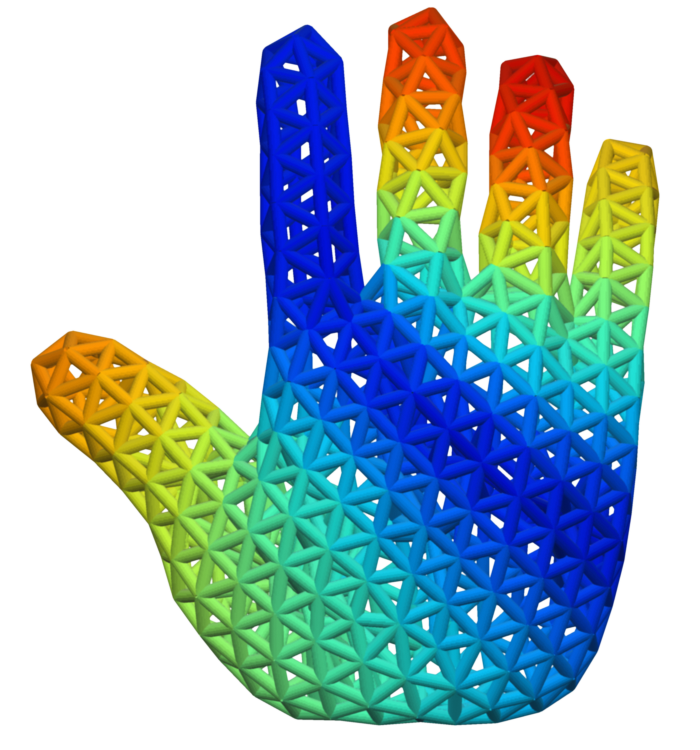
\includegraphics[width=.48\linewidth]{Figures/eigen/eigen_frame_uni.png}
  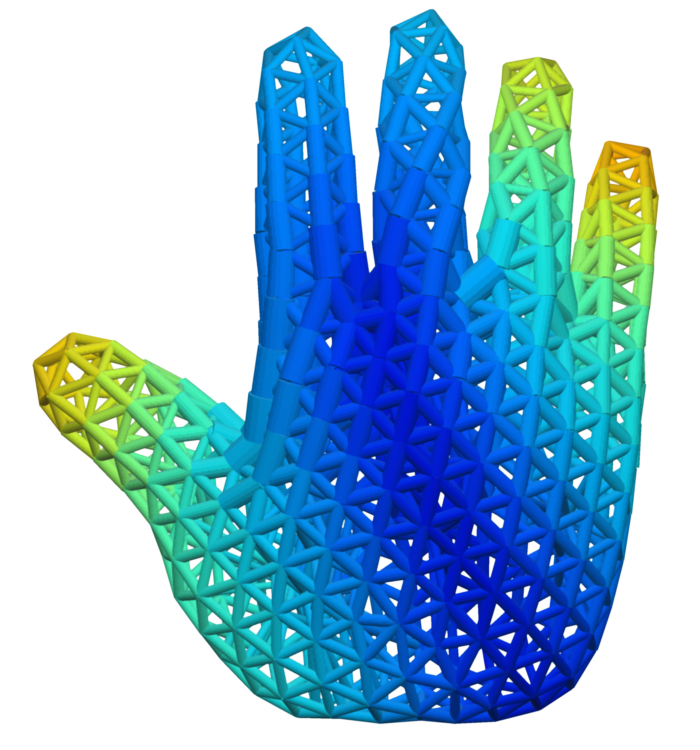
\includegraphics[width=.48\linewidth]{Figures/eigen/eigen_frame_ours.png}
  \caption{\label{fig:result-validation-max-deformation}
  Maximum deformation distribution on different structures.
            Left: uniform frame; Right: our optimized structure.
            The magnitude of maximum deformation on our resulting structure is much smaller than that on the uniform frame. }
\end{figure}



\paragraph{Deformation under various forces}
We also test the result by several cases of $f$ acting on the object.
For example, two fingers of a hand model are pushed to simulate the action of pinching (see Figure \ref{fig:result-validation-sample-force}).
More tests are done for the hand model under 10 different force conditions; see the table for
comparison between the uniform structures and the optimized ones.


\begin{figure}[h]
  \centering
%  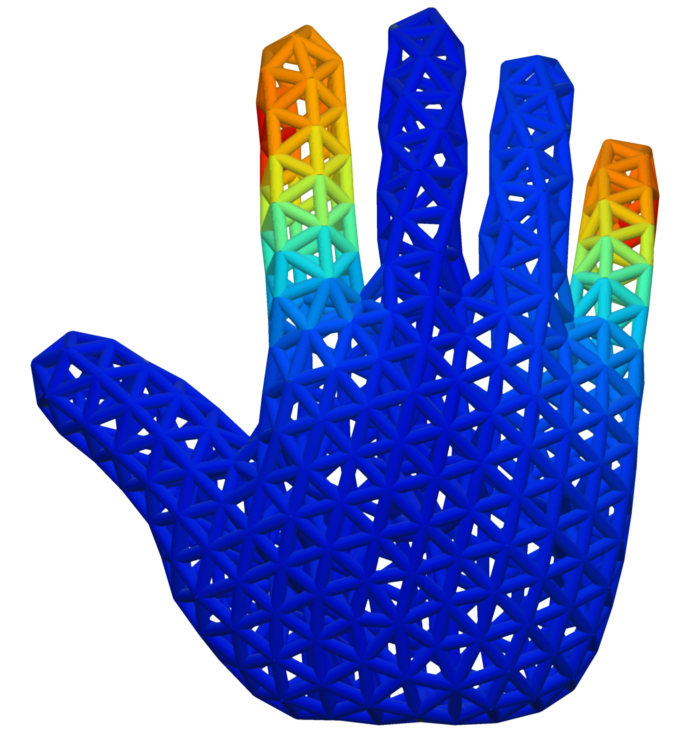
\includegraphics[width=.24\linewidth]{Figures/hand/hand_case1_frame_uni.png}
%  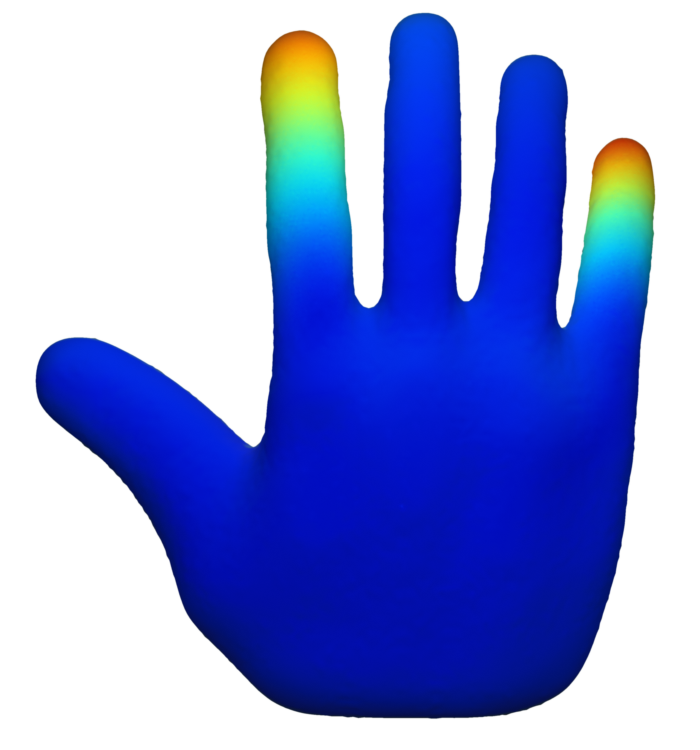
\includegraphics[width=.24\linewidth]{Figures/hand/hand_case1_solid_uni.png}
%  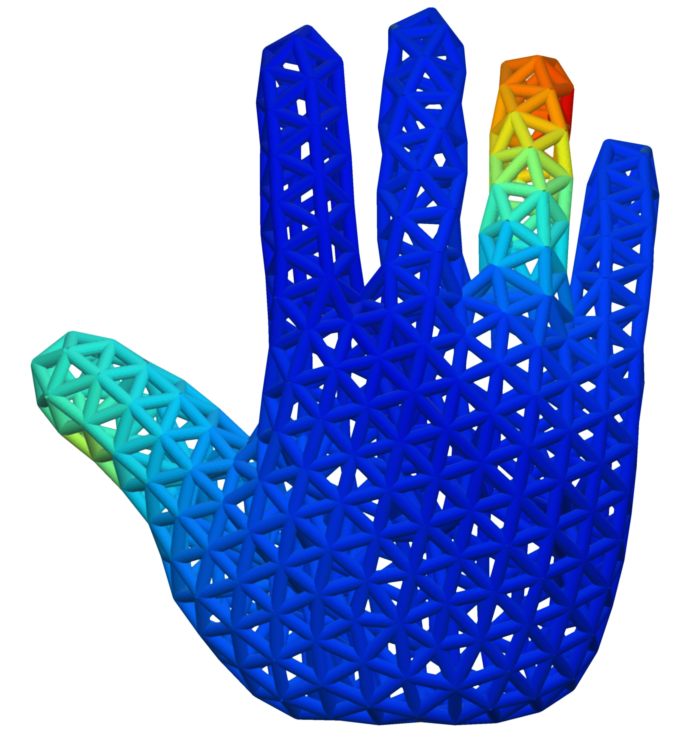
\includegraphics[width=.24\linewidth]{Figures/hand/hand_case2_frame_uni.png}
%  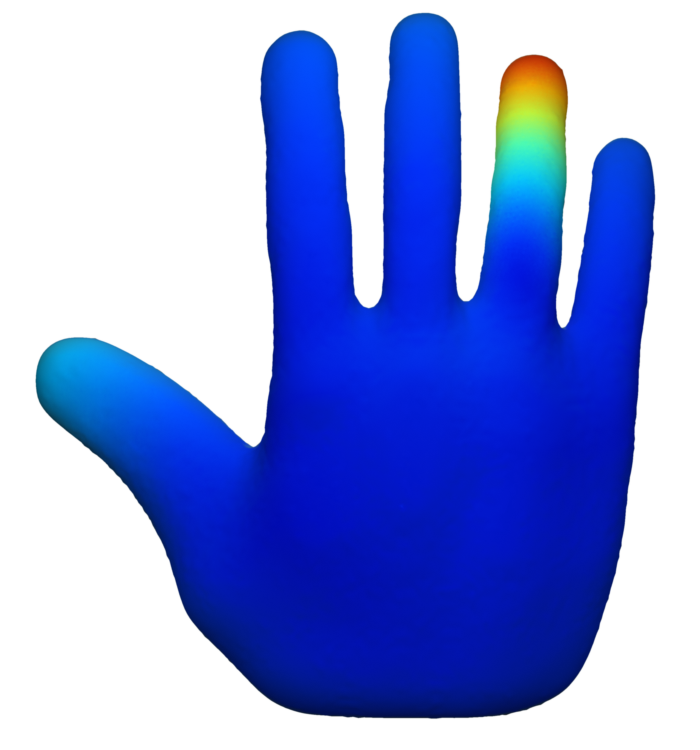
\includegraphics[width=.24\linewidth]{Figures/hand/hand_case2_solid_uni.png} \\
%  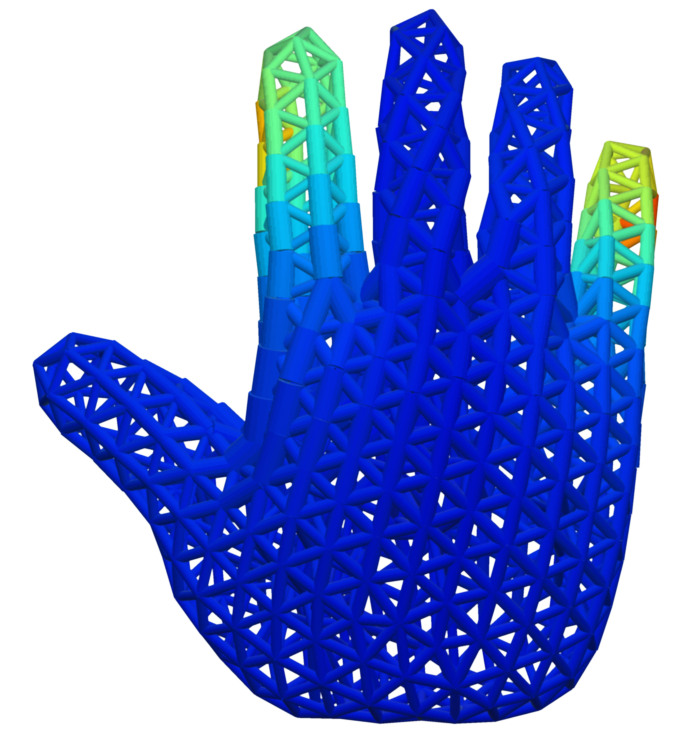
\includegraphics[width=.24\linewidth]{Figures/hand/hand_case1_frame_ours.png}
%  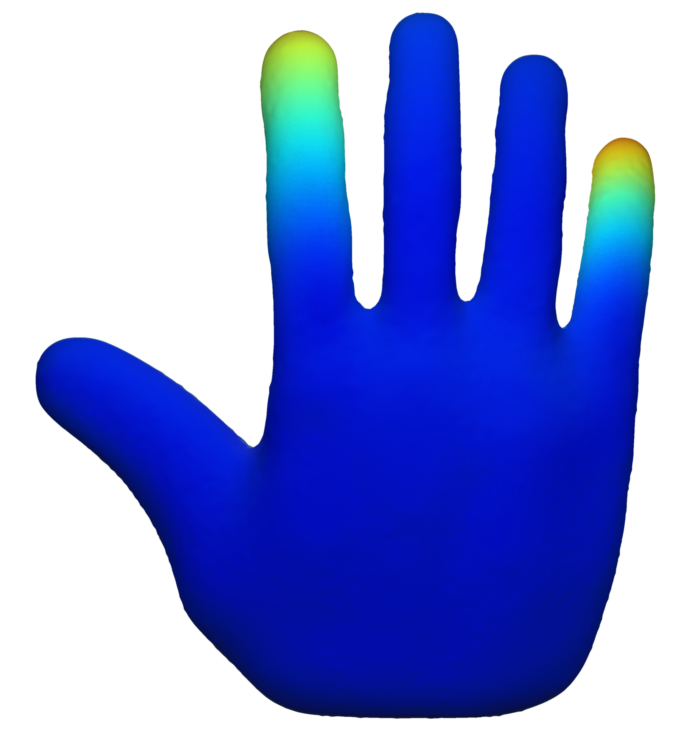
\includegraphics[width=.24\linewidth]{Figures/hand/hand_case1_solid_ours.png}
%  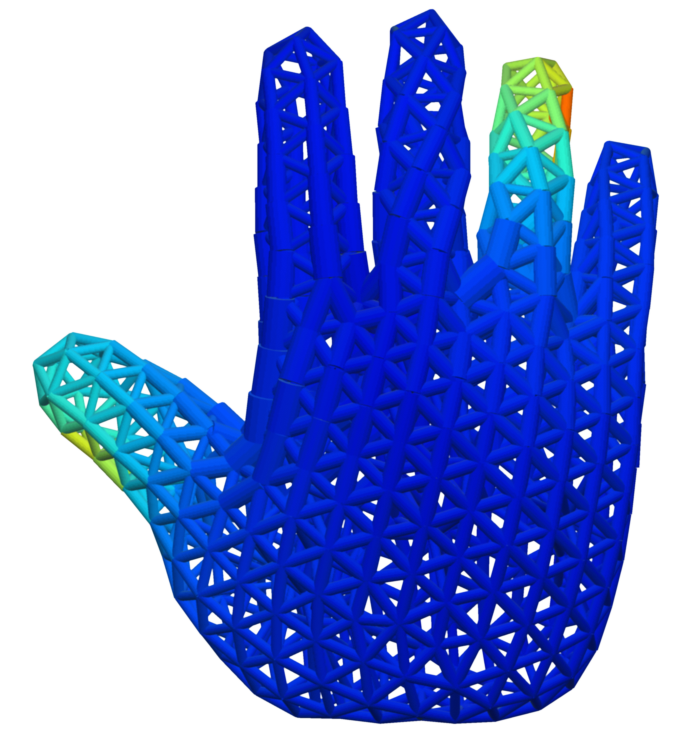
\includegraphics[width=.24\linewidth]{Figures/hand/hand_case2_frame_ours.png}
%  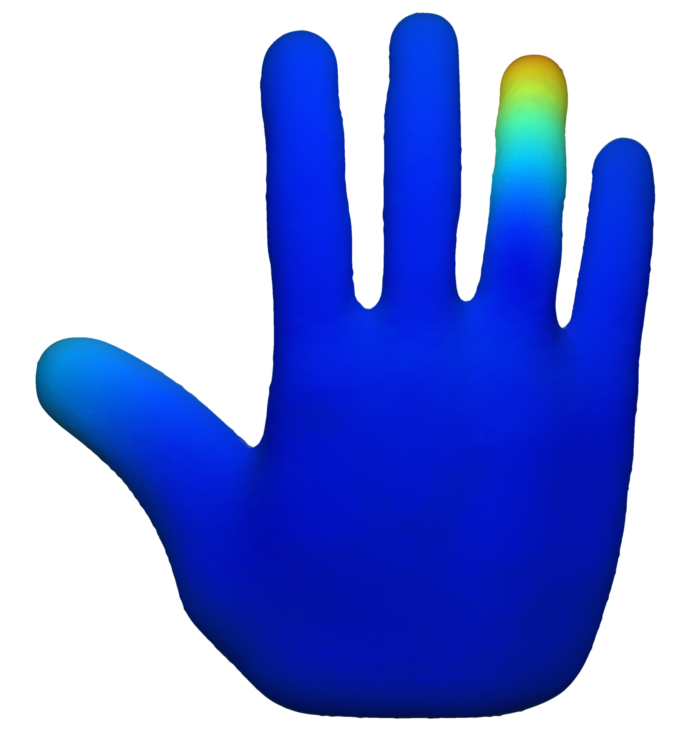
\includegraphics[width=.24\linewidth]{Figures/hand/hand_case2_solid_ours.png}
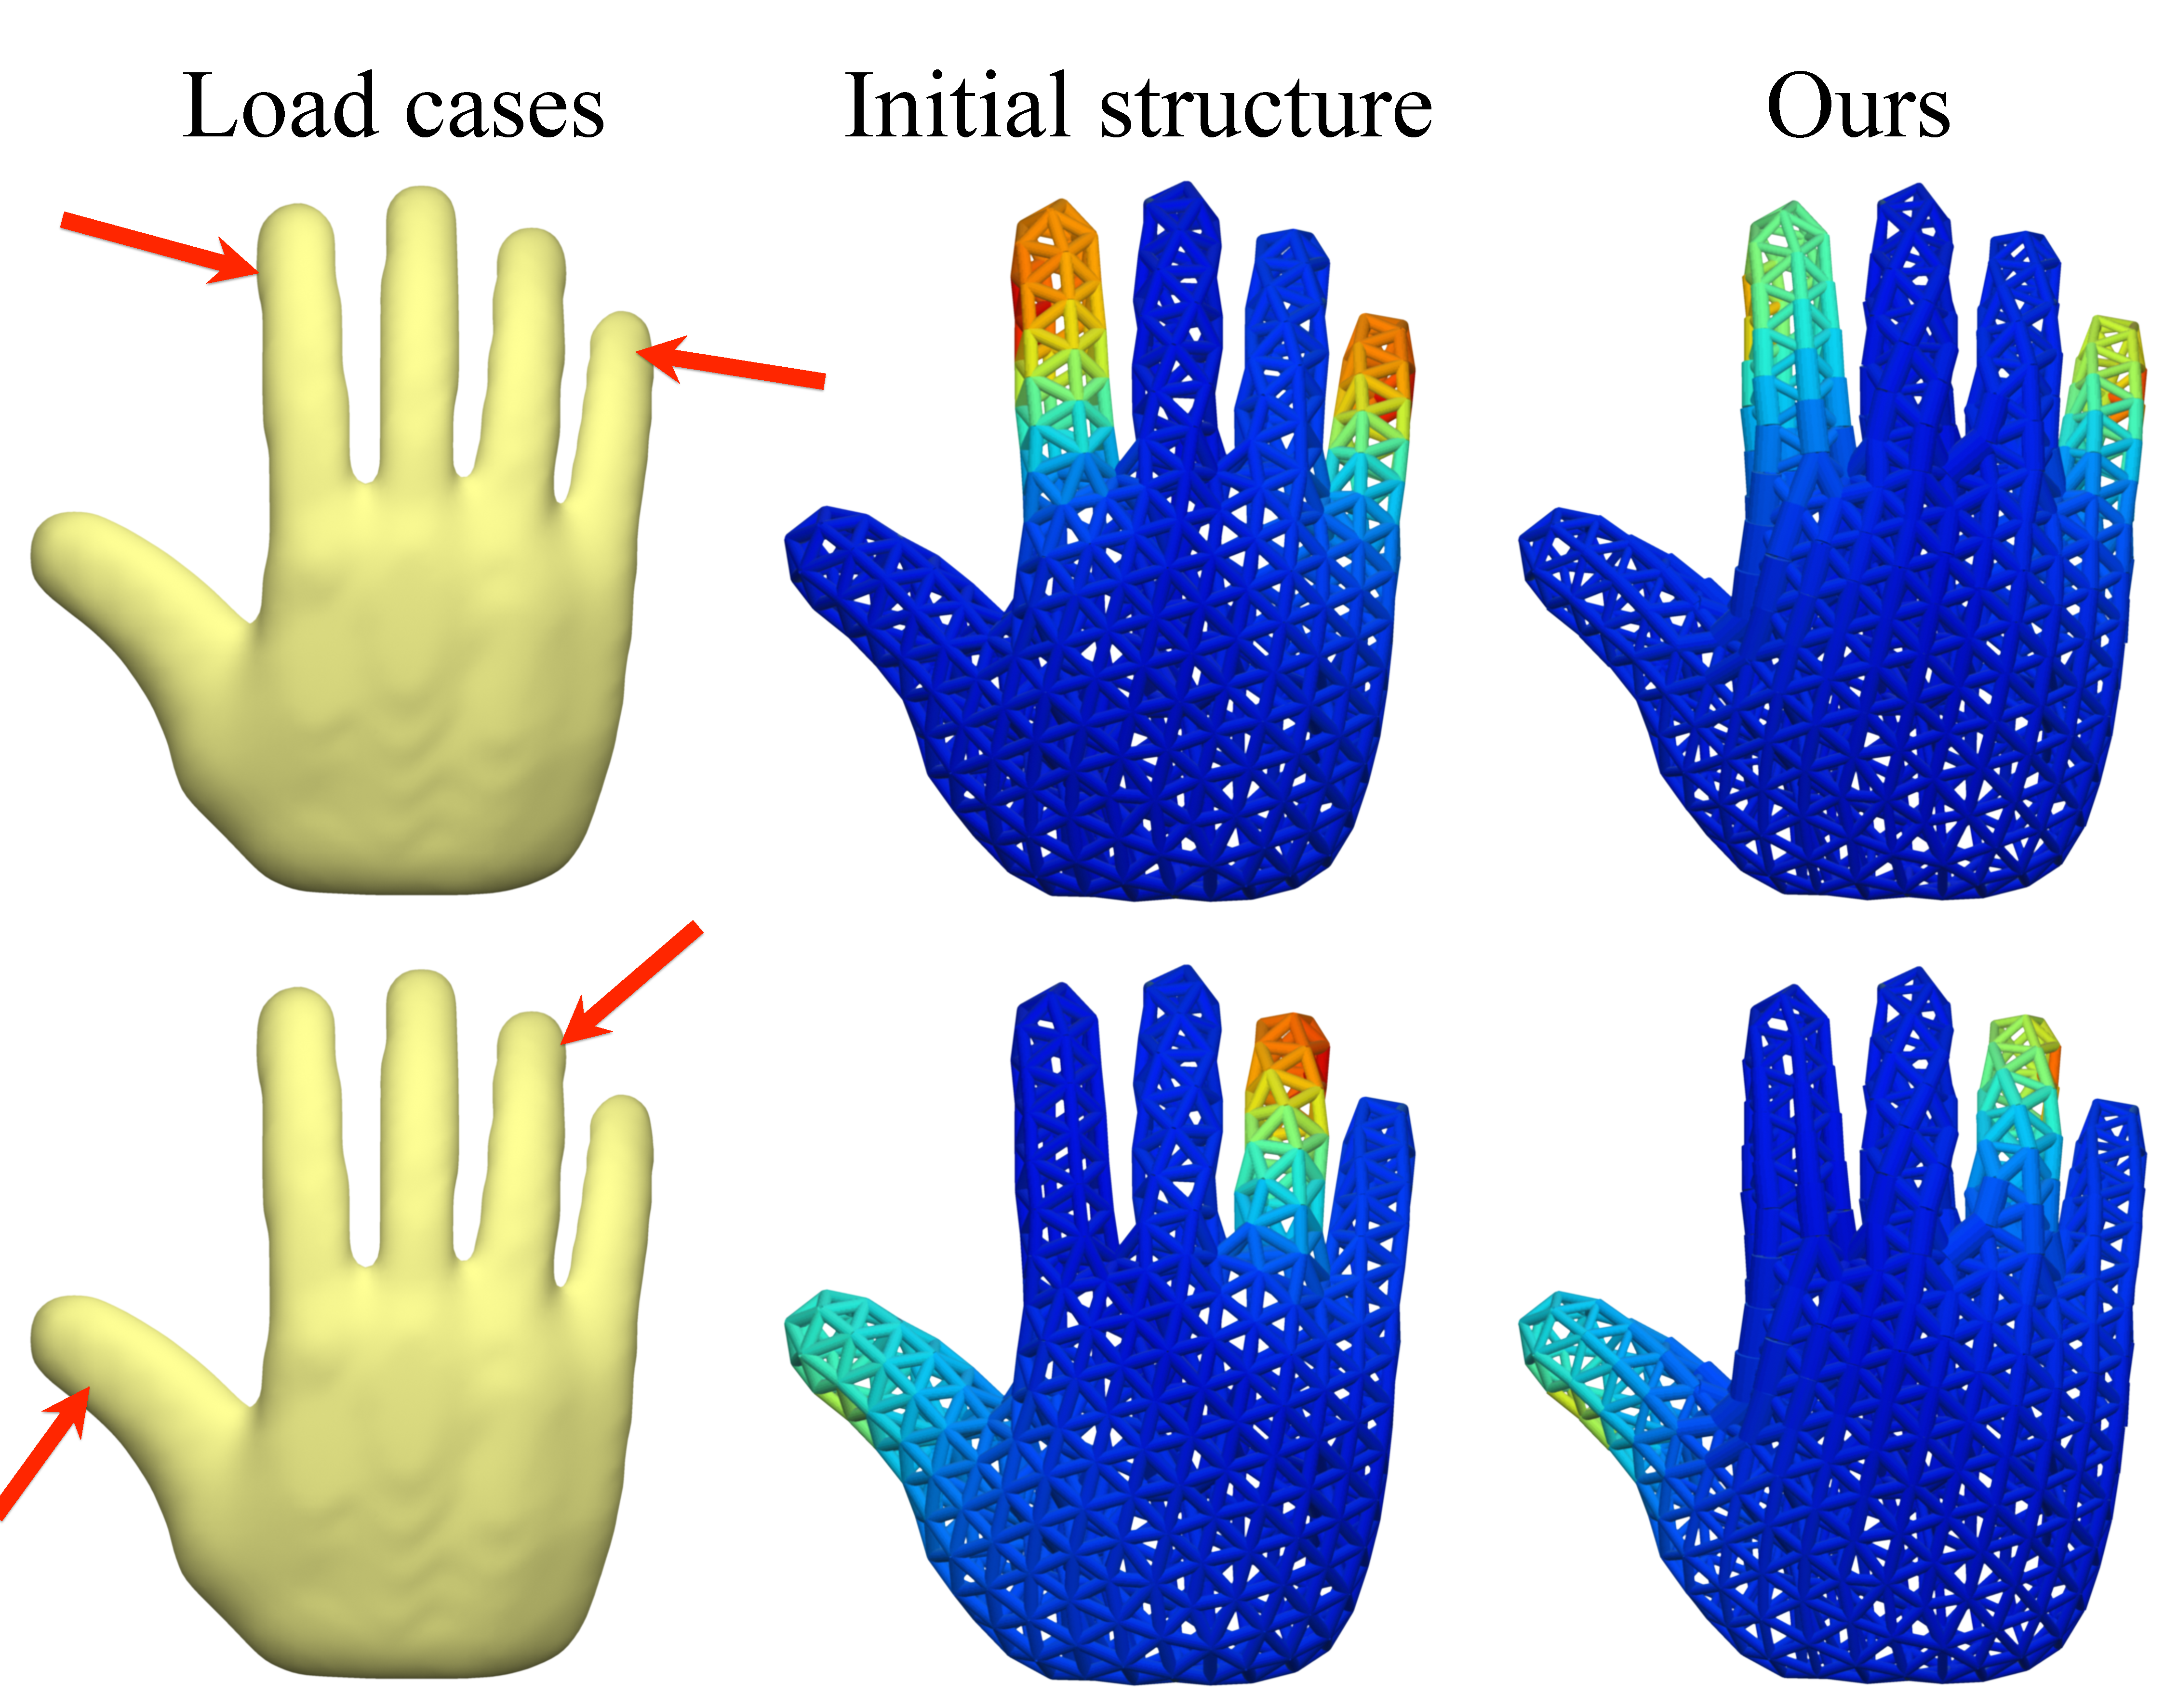
\includegraphics[width=\linewidth]{Figures/hand/hand.pdf}
  \caption{\label{fig:result-validation-sample-force} Deformation distribution on different structures (
            %
            Simulation of the action of pinching on the hand model.
            Left: the input model (top) and the printed object of our result (bottom).
            Middle: deformation on the frame structure with uniform radii (top) and our optimized frame (bottom).
            Right: deformation on the solid structure generated from the uniform frame (top) and the solid structure generated from our optimized frame (bottom), both structures have the same volume.
            The red arrows shown on the printed object bottom left indicate that the deformation is simulated under a pair of forces.
            In the Middle and Right columns hotter color refers to a larger value of deformation and cooler color refers to a smaller value of deformation.
            }
\end{figure}


\begin{table}[htb]
\caption{\label{tab:result-validation}Statistics of the simulation tests for the hand model.
    10 records of displacement (disp., in mm) and stress (strs., in MPa) are listed.
    First two rows are the results of uniform frame and the last two rows are our results .}
\centering
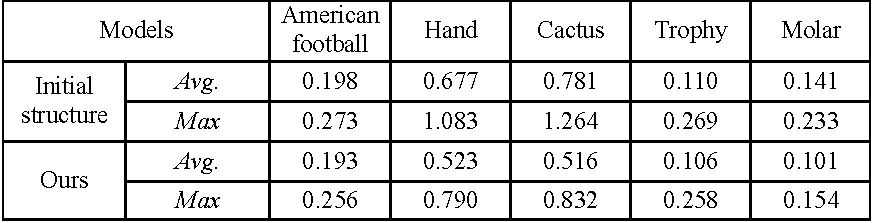
\includegraphics[width=\linewidth]{Tables/table1}
%\tiny
%%\begin{small}
%\begin{tabular}{|c|c|c|c|c|c|c|c|c|c|c|c|c|c|}
% \hline
% test &              &   1 & 2   & 3   &  4   & 5    & 6     & 7     & 8     & 9     & 10    &  mean & var  \\
%\hline
%\multirow{2}{*} {adp.}
%             & disp. & 1.1 & 1.2 & 0.4 & 0.08 & 0.96 & 0.09  & 0.68  & 0.6   & 0.3   & 0.4   & 0.58  & 0.16 \\
% \hhline{~-------------}
%             & strs.       & 25  & 29  & 13  & 19   & 20   & 12    & 17    & 22    & 8.1   & 8.5   & 17.36 & 48.57\\
% \hline \multirow{2}{*}{uni.}
%             & disp. & 1.3 & 1.7 & 0.76& 0.08 & 1.2  & 0.14  & 0.7   & 0.83  & 0.39  & 0.55  & 0.765 & 0.27 \\
% \hhline{~-------------}
%             & strs.       & 35  & 43  & 17  & 19   & 27   & 15    & 22    & 21    & 12    & 12    & 22.30 & 102.0\\
% \hline
%\end{tabular}
%%\end{small}
\end{table}


%\begin{figure}[htb]
%  \centering
%  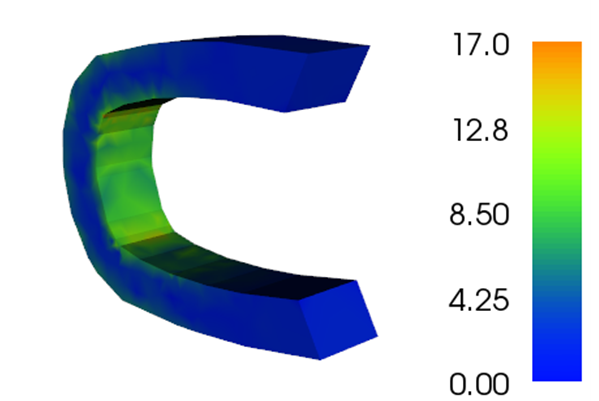
\includegraphics[width=0.45\linewidth]{Figures/results/stress1.png}
%  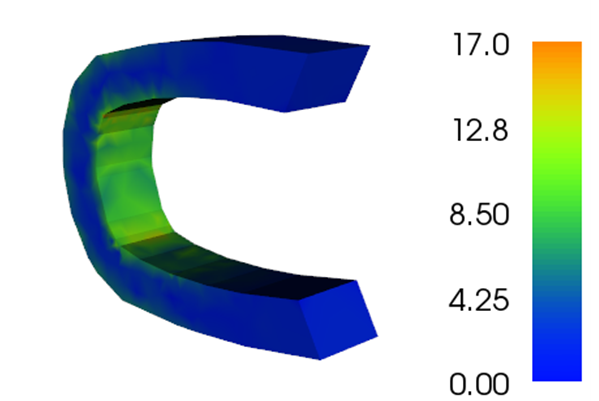
\includegraphics[width=0.45\linewidth]{Figures/results/stress2.png}
%  \caption{\label{fig:simul-stress-horseshoe}
%           Stress distribution comparison.}
%\end{figure}


\paragraph{Structural optimization for several models}
Table~\ref{tab:result-statistics} shows the performance statistics of applying our method to different models.
`Ratio' denotes the ratio of our optimized structure volume to the whole volume of the model.
For the examples in consideration, this ratio is set to $30\%$ in average.
For models with highly curved surfaces, we set higher bound for the volume since adaptively thickening the surface cost more volume than other models.


%\paragraph{Statistics}
%Table \ref{tab:result-statistics} shows the statistics of applying our method to different models.
%'Ratio' denotes the ratio of total volume. The material saving is about 70$\%$ in average.
%For models with highly curved surfaces, the volume cost is higher since adaptively thickening the surface
%cost more volume than other models.

\begin{table}[htb]
\caption{\label{tab:result-statistics} Statistics of our method on various models. \#V and \#E are the number of nodes and edges, respectively. $Time$ is the computing time of our optimization process (in minutes). $Vol$ is the volume (in $mm^3$) of the resulting structure. $Ratio$ is the ratios of structure volume to the whole volume of the model. }
\centering
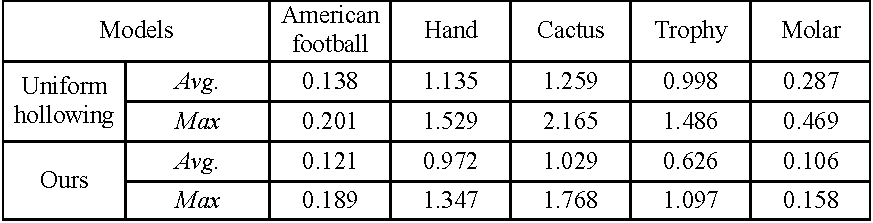
\includegraphics[width=\linewidth]{Tables/table2}
%
%\bigskip
%\begin{small}
%\tiny
%\begin{tabular}{|c|c|c|c|c|c|c|c|c|c|}
% \hline
% Model      & \#V & \#E &  $T_i$   &  $T_o$  & $T_p$ &  $V_u$  & $R_u$    &   $V_r$ & $R_r$ \\ \hline
% Copa       & 80    & 368   &  1                &   2.3             &  15               &  77750                &   25$\%$  &   82801       &   26.6$\%$ \\ \hline
% Cactus     & 160   & 669   &  2                &   0.9             &  12               &  7528                 &   40$\%$  &   10096       &   45.3$\%$ \\ \hline
% Hand       & 500   & 1373  &  5                &   7.5             &  15               &  31075                &   45$\%$  &   31161       &   45.1$\%$ \\ \hline
% Football   & 50    & 267   &  0.5              &   0.2             &  7                &  74156                &   20$\%$  &   76297       &   20.5$\%$ \\ \hline
% Head       & 80    & 376   &  1                &   1.5             &  11               &  69241                &   20$\%$  &   72203       &   20.8$\%$ \\ \hline
%\end{tabular}
%%\end{small}
\end{table}




